\documentclass[11pt]{amsart}

\usepackage[margin=1.08in]{geometry}
\usepackage{amsmath,amssymb,amsthm}
\usepackage{enumitem}
\usepackage{graphicx}
\usepackage[hidelinks]{hyperref}

\newtheorem{theorem}{Theorem}
\newtheorem{lemma}{Lemma}
\theoremstyle{remark}
\newtheorem{remark}{Remark}

\newcommand{\bbT}{\mathbb T}
\newcommand{\bbZ}{\mathbb Z}
\newcommand{\calA}{\mathcal A}
\newcommand{\DPP}{\operatorname{DPP}}

\title{The high-exponent Dunford--Pettis question for $A_2^r(\mathbb Z)$}
\author{Agent lane 04}
\date{Run \texttt{fa\_banach\_001}, 2026-06-29}

\begin{document}
\maketitle

\section*{Status}

This packet gives a scoped full answer to the $G=\mathbb Z$, $p=2$ part of a
question in Granirer \cite{Granirer2020}.  The source asks whether
$A_p^r(G)$ has the Dunford--Pettis property when
$r>\max\{p,p'\}$, even for $G=\mathbb Z$ and $p=2$.  The answer is:
\[
  A_2^r(\mathbb Z) \text{ fails the Dunford--Pettis property for every }
  1<r<\infty,
\]
and in particular for every finite $r>2$.  The endpoint
$r=\infty$ is different: by definition $A_2^\infty(\mathbb Z)=A_2(\mathbb Z)$,
which is isometric to $L^1(\mathbb T)$ and therefore has the
Dunford--Pettis property.

\section*{Source question}

After proving the DPP failure for discrete $G$ in the range
$1<r\leq \max\{p,p'\}$, the source asks:

\begin{quote}
It is not clear to us if $A_p^r(G)$ has the DPP if
$r>\max\{p,p'\}$ in case $G$ is discrete, or even if $G=\mathbb Z$ and
$p=2$.
\end{quote}

\begin{center}
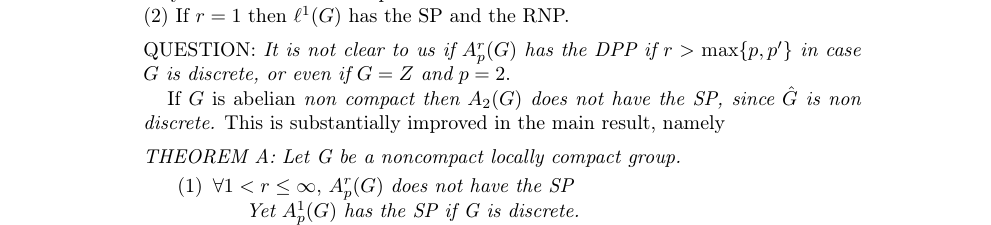
\includegraphics[width=0.94\textwidth]{figures/dpp_question_crop.png}
\end{center}

\section*{Idea of the proof}

For $G=\mathbb Z$, the Fourier algebra is simply the Fourier transform of
$L^1(\mathbb T)$.  For finite $r$, the space $A_2^r(\mathbb Z)$ is the graph
space of the Fourier coefficient map
\[
   f\longmapsto \widehat f
\]
inside $L^1(\mathbb T)\oplus \ell^r(\mathbb Z)$, with norm
\[
   \|f\|_{1}+\|\widehat f\|_{r}.
\]
The monomials $z^n$ are weakly null in $L^1(\mathbb T)$, while the unit vectors
$e_n$ are weakly null in $\ell^r$ for $1<r<\infty$.  Thus the corresponding
elements of $A_2^r(\mathbb Z)$ are weakly null.  On the dual side, the
coordinate functionals are weakly null because they come from the weakly null
coordinate basis of $\ell^{r'}$.  Their pairings with the matching monomials
stay equal to one, which is exactly the standard obstruction to the
Dunford--Pettis property.

\section*{Proof}

\begin{theorem}
Let $1<r<\infty$.  Then $A_2^r(\mathbb Z)$ does not have the
Dunford--Pettis property.
\end{theorem}

\begin{proof}
Use normalized Haar measure on $\mathbb T$.  Under the Fourier transform,
$A_2(\mathbb Z)$ is isometric to $L^1(\mathbb T)$, and
\[
 A_2^r(\mathbb Z)
   =\{ \widehat f : f\in L^1(\mathbb T),\ \widehat f\in \ell^r(\mathbb Z)\}
\]
with norm $\|\widehat f\|_{A_2^r}=\|f\|_1+\|\widehat f\|_{\ell^r}$.
Equivalently, it is the graph subspace
\[
 X_r=\{(f,\widehat f): f\in L^1(\mathbb T),\ \widehat f\in\ell^r(\mathbb Z)\}
      \subset L^1(\mathbb T)\oplus_1 \ell^r(\mathbb Z).
\]

For $n\in\mathbb Z$, let $x_n\in X_r$ correspond to the Fourier monomial
$z^n$; in graph notation,
\[
        x_n=(z^n,e_n),
\]
where $e_n$ is the $n$th coordinate vector of $\ell^r(\mathbb Z)$.
The sequence $(z^n)$ is weakly null in $L^1(\mathbb T)$: for every
$g\in L^\infty(\mathbb T)\subset L^1(\mathbb T)$, the Riemann--Lebesgue lemma
gives
\[
        \int_{\mathbb T} z^n g(z)\,dm(z)\longrightarrow 0
\]
as $|n|\to\infty$.  Also $(e_n)$ is weakly null in $\ell^r(\mathbb Z)$ since
$1<r<\infty$.  Hence $(x_n)$ is weakly null in the graph subspace $X_r$.

Let $\varphi_n\in X_r^*$ be the restriction to $X_r$ of the $n$th coordinate
functional on the $\ell^r$ summand:
\[
        \varphi_n(f,\widehat f)=\widehat f(n).
\]
The coordinate basis of $\ell^{r'}(\mathbb Z)=(\ell^r(\mathbb Z))^*$ is weakly
null because $1<r'<\infty$.  Therefore $(\varphi_n)$ is weakly null in
$X_r^*$, being the image of a weakly null sequence under the adjoint of the
inclusion $X_r\hookrightarrow L^1(\mathbb T)\oplus_1\ell^r(\mathbb Z)$.

But the pairings do not tend to zero:
\[
        \varphi_n(x_n)=e_n(n)=1\qquad(n\in\mathbb Z).
\]
Thus there are weakly null sequences $(x_n)\subset X_r$ and
$(\varphi_n)\subset X_r^*$ whose scalar pairings stay equal to one.  This is
precisely a failure of the Dunford--Pettis property.
\end{proof}

\begin{theorem}
For the high-exponent question with $G=\mathbb Z$ and $p=2$:
\[
 A_2^r(\mathbb Z) \text{ has the DPP}
 \quad\Longleftrightarrow\quad
 r=1 \text{ or } r=\infty
\]
within the source's range $1\le r\le\infty$.
\end{theorem}

\begin{proof}
For $1<r<\infty$, this is the previous theorem.  For $r=1$, the source already
records that $A_p^1(G)=\ell^1(G)$ for discrete $G$, hence has the Schur
property and therefore the DPP.  For $r=\infty$, the definition gives
$A_2^\infty(\mathbb Z)=A_2(\mathbb Z)$.  Since
$A_2(\mathbb Z)\cong L^1(\mathbb T)$ and $L^1(\mu)$ has the Dunford--Pettis
property for every measure $\mu$, the endpoint $r=\infty$ has the DPP.
\end{proof}

\section*{Limitations}

This settles the $G=\mathbb Z$, $p=2$ Dunford--Pettis subquestion.  It does not
settle whether $A_2^r(\mathbb Z)$ has the Radon--Nikodym property for finite
$r>2$, nor the corresponding questions for $G=\mathbb R$, nor the source
conjecture that $A_2^r(G)$ has the DPP for connected semisimple Lie groups
with finite center and $r>2$.

\section*{Novelty and verification notes}

\begin{itemize}[leftmargin=*]
\item Local run indexes were searched for \texttt{2006.13021},
\texttt{A\_2\^{}r(Z)}, \texttt{Dunford-Pettis}, \texttt{A\_p\^{}r(G)}, and
related Fourier-algebra phrases.  No prior packet for this source or exact
question was found.
\item Bounded web search on 2026-06-29 for
``$A_2^r(Z)$ Dunford Pettis Property'', ``$A_p^r(G)$ Dunford-Pettis Z'', and
the source title found only the source paper, not a later answer.
\item The proof uses only the standard Fourier identification
$A_2(\mathbb Z)\cong L^1(\mathbb T)$, the Riemann--Lebesgue lemma, reflexivity
of $\ell^r$ for $1<r<\infty$, and the classical fact that $L^1(\mu)$ has the
Dunford--Pettis property.
\end{itemize}

\section*{Human review recommendation}

Review as a short, likely valid scoped full solution.  The key point to check
is that weak convergence in the graph subspace follows from weak convergence
in the ambient direct sum; this is immediate by Hahn--Banach extension of
functionals from the subspace.

\begin{thebibliography}{9}

\bibitem{Granirer2020}
E. E. Granirer,
\emph{Geometric Properties of some Banach Algebras related to the Fourier
algebra on Locally Compact Groups},
arXiv:2006.13021, 2020.
\url{https://arxiv.org/abs/2006.13021}

\bibitem{Diestel1980}
J. Diestel,
\emph{A survey of results related to the Dunford--Pettis property},
Contemporary Mathematics 2, American Mathematical Society, 1980.

\end{thebibliography}

\end{document}
